\documentclass[tikz,border=8pt]{standalone}
\usepackage{amsmath}
\usetikzlibrary{arrows.meta,calc}
\usepackage{xcolor}
\definecolor{deepblue}{RGB}{0,0,139} % 짙은 파랑

\begin{document}
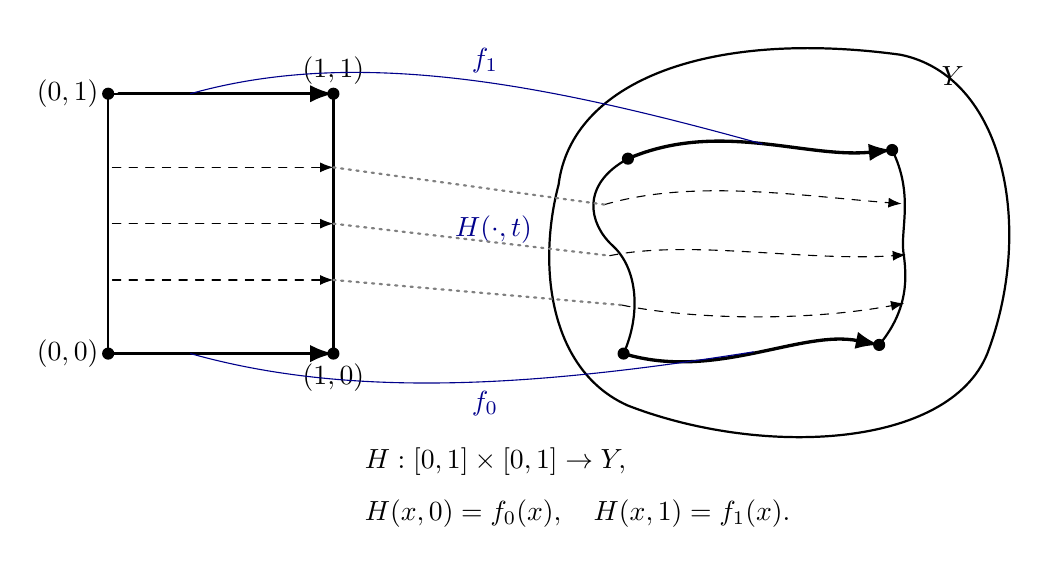
\begin{tikzpicture}[>=Latex, line cap=round, line join=round, scale=1.1]

%==================================================
% Left square [0,1]x[0,1]
%==================================================
\coordinate (A) at (0,0);
\coordinate (B) at (0,3);
\coordinate (C) at (2.6,3);
\coordinate (D) at (2.6,0);

\draw[thick] (A) rectangle (C);

% Corner points: black
\foreach \p in {A,B,C,D}{
  \fill[black] (\p) circle (0.07);
}

% Labels
\node[left]  at (A) {$(0,0)$};
\node[left]  at (B) {$(0,1)$};
\node[above] at (C) {$(1,1)$};
\node[below] at (D) {$(1,0)$};

%--------------------------------------------------
% X-region arrows: unify arrowhead x-position
%--------------------------------------------------
\draw[very thick, ->] (0.12,3) -- (1.55,3) -- (2.60,3);
\draw[dashed,    ->] (0.05,2.15) -- (1.55,2.15) -- (2.60,2.15);
\draw[dashed,    ->] (0.05,1.50) -- (1.55,1.50) -- (2.60,1.50);
\draw[dashed,    ->] (0.05,0.85) -- (1.55,0.85) -- (2.60,0.85);
\draw[very thick, ->] (0.12,0) -- (1.55,0) -- (2.60,0);

%==================================================
% Right codomain Y
%==================================================
\draw[thick]
  (5.20,1.95)
  .. controls (5.35,3.15) and (6.95,3.75) .. (9.15,3.45)
  .. controls (10.35,3.20) and (10.70,1.45) .. (10.15,0.00)
  .. controls (9.70,-1.10) and (7.55,-1.20) .. (6.00,-0.60)
  .. controls (5.10,-0.20) and (4.95,1.00) .. (5.20,1.95);

\node at (9.75,3.20) {$Y$};

% Inner boundary corner points
\coordinate (P1) at (6.0,2.25);   % top-left
\coordinate (P2) at (9.05,2.35);  % top-right
\coordinate (P3) at (8.9,0.10);   % bottom-right
\coordinate (P4) at (5.95,0.00);  % bottom-left

% Black marked points
\foreach \p in {P1,P2,P3,P4}{
  \fill[black] (\p) circle (0.07);
}

% Left wavy side
\draw[thick]
  (P1)
  .. controls (5.45,1.95) and (5.55,1.50) .. (5.82,1.25)
  .. controls (6.12,0.98) and (6.15,0.45) .. (P4);

% Right wavy side
\draw[thick]
  (P2)
  .. controls (9.30,1.85) and (9.15,1.45) .. (9.18,1.18)
  .. controls (9.22,0.90) and (9.25,0.52) .. (P3);

% Top solid image
\draw[very thick, ->]
  (P1) .. controls (7.05,2.70) and (8.05,2.25) .. (P2);

% Bottom solid image
\draw[very thick, ->]
  (P4) .. controls (7.00,-0.32) and (8.00,0.28) .. (P3);

%==================================================
% Three dashed curves inside Y
%  each one resembles the nearby thick curve
%==================================================
\coordinate (L1) at (5.73,1.72);
\coordinate (R1) at (9.16,1.73);

\coordinate (L2) at (5.79,1.13);
\coordinate (R2) at (9.21,1.14);

\coordinate (L3) at (5.93,0.56);
\coordinate (R3) at (9.19,0.58);

% Top dashed curve: closer to the top thick curve
\draw[dashed, ->]
  (L1) .. controls (6.75,2.02) and (8.00,1.82) .. (R1);

% Middle dashed curve: intermediate shape
\draw[dashed, ->]
  (L2) .. controls (6.72,1.32) and (8.05,1.06) .. (R2);

% Bottom dashed curve: closer to the bottom thick curve
\draw[dashed, ->]
  (L3) .. controls (6.70,0.40) and (8.00,0.36) .. (R3);
%==================================================
% Connectors from square to codomain
%==================================================

% Start points at the middle of the thick arrows
\coordinate (Mtop) at (0.95,3);
\coordinate (Mbot) at (0.95,0);

% Endpoints moved to the middle of the thick image curves
\coordinate (Q1) at (7.55,2.42);
\coordinate (Q0) at (7.45,0.02);

% Top solid-to-solid connector (f1): more curved
\draw[deepblue, thin]
  (Mtop) .. controls (2.90,3.55) and (5.10,3.10) .. (Q1);
\node[deepblue] at (4.35,3.38) {$f_1$};

% Bottom solid-to-solid connector (f0): more curved
\draw[deepblue, thin]
  (Mbot) .. controls (2.90,-0.55) and (5.10,-0.35) .. (Q0);
\node[deepblue] at (4.35,-0.58) {$f_0$};

% Label between f1 and f0
\node[deepblue] at (4.45,1.43) {$H(\cdot,t)$};

% Dashed-to-dashed connectors
\draw[dotted, gray, thick] (2.60,2.15) -- (L1);
\draw[dotted, gray, thick] (2.60,1.50) -- (L2);
\draw[dotted, gray, thick] (2.60,0.85) -- (L3);

%==================================================
% Formula moved left
%==================================================
\node[anchor=west] at (2.85,-1.25) {$H:[0,1]\times[0,1]\to Y,$};
\node[anchor=west] at (2.85,-1.85) {$H(x,0)=f_0(x),\quad H(x,1)=f_1(x).$};

\end{tikzpicture}
\end{document}